\documentclass[11pt]{article}
\usepackage{setspace}
\usepackage[a4paper,margin=1in]{geometry}
\geometry{margin=0.85in}
\setstretch{1.0}
\usepackage{graphicx}
\usepackage{array}
\usepackage{setspace}
\usepackage{parskip}
\usepackage{ragged2e}

\pagestyle{empty}
\setstretch{1.05}

\begin{document}


% Title
\begin{center}
    {\Large \textbf{Job Application}} \\[3cm]
    
    {\Huge \textbf{Zhongli Wang}} \\[0.4cm]
    
    {\LARGE Application for Research Assistant}
\end{center}

\vspace{0.6cm}

% Large picture in the middle
\begin{center}
    \IfFileExists{../zhongli-wang-profile.jpg}{
        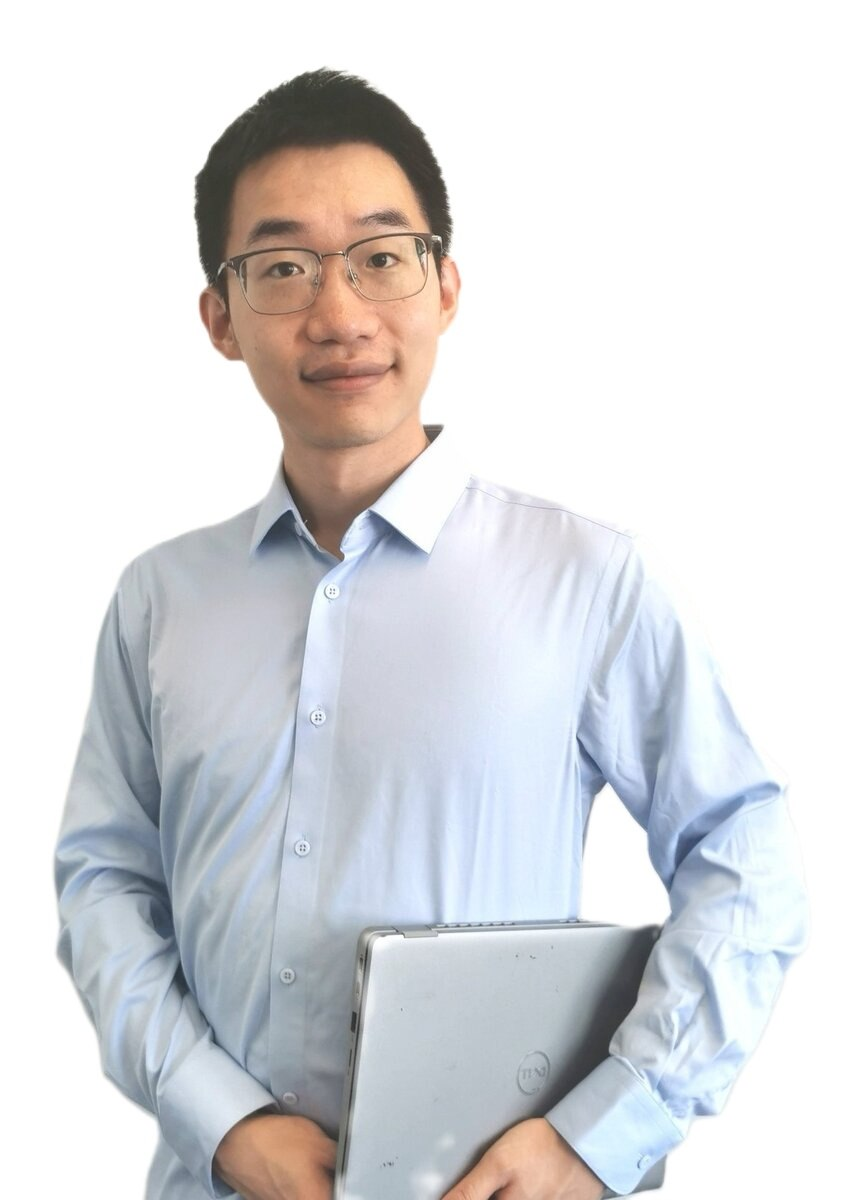
\includegraphics[
            width=0.55\textwidth,
            height=0.45\textheight,
            keepaspectratio
        ]{../zhongli-wang-profile.jpg}
    }{
        \vspace{0.45\textheight}
    }
\end{center}

\vspace{0.7cm}

% \vspace{3cm}


% Personal details
\begin{center}
\renewcommand{\arraystretch}{1.35}
\begin{tabular}{>{\bfseries}p{4.2cm} p{8.5cm}}


Address: & Astastrasse 22, 33617 Bielefeld, Germany \\

Number: & +49 160 9541 6015 \\

Email: & nkwangzhongli@gmail.com \\
\end{tabular}
\end{center}

\vfill

% \begin{center}
%     \small Last updated: \today
% \end{center}
\newpage
\enlargethispage{4\baselineskip}

\begin{flushright}
Zhongli Wang \\
Astastrasse 22 \\
33617 Bielefeld\\
Germany \\
\end{flushright}

\vspace{0.1cm}

\vspace{0.1cm}

\noindent
Hang Seng University of Hong Kong \\
Department of Computer Science \\
Hong Kong

\vspace{0.12cm}

\noindent
\textbf{Application for Research Assistant}

\vspace{0.1cm}

\noindent Dear HSUHK Hiring Committee,

I am writing to apply for the Research Assistant position in the Department of Computer Science at Hang Seng University of Hong Kong, working on the project ``Graph Neural Networks Assisted Dynamic Task Offloading in Internet of Vehicles.'' I have successfully completed my Ph.D. in Economics at Bielefeld University (defense: September 21, 2026) and hold an M.A. in Business and Economics with a minor in Data Science. My doctoral research in computational economics and agent-based modeling has developed strong analytical, mathematical, and programming skills that align well with the research requirements.

I am particularly interested in this position because it combines deep learning, mobile edge computing, and graph neural networks—areas where my research background and technical expertise are directly applicable. My relevant qualifications include:

\begin{itemize}
    \item \textbf{Deep learning and neural networks:} My doctoral research develops agent-based computational models and applies machine learning methods (XGBoost, Random Forest, Neural Networks) to large-scale datasets. I have hands-on experience implementing and training neural network models for economic prediction and optimization tasks, which provides a strong foundation for working with graph neural networks.
    \item \textbf{Mathematical and analytical skills:} My Ph.D. training emphasizes rigorous mathematical modeling, statistical analysis, and algorithmic thinking. I have developed computational models to analyze complex systems, optimize decision-making under uncertainty, and validate theoretical predictions against empirical data—skills directly transferable to GNN-based task offloading optimization.
    \item \textbf{Programming proficiency:} I am proficient in Python, R, and have experience with data processing libraries (pandas, NumPy, scikit-learn). I have implemented computational models from scratch, managed large datasets, and developed reproducible research workflows. I am confident in my ability to quickly master GNN frameworks and mobile edge computing tools.
    \item \textbf{Research and academic writing:} I have authored peer-reviewed publications, prepared technical reports, and presented research at international conferences. I have strong writing skills and experience translating complex technical concepts clearly, which will support effective reporting of experimental results and academic paper drafting.
\end{itemize}

I am highly motivated to contribute to cutting-edge research in graph neural networks and mobile edge computing. I am eager to work independently on research tasks while collaborating effectively with the research team, and to develop expertise in this emerging field. My analytical mindset, strong work ethic, and commitment to rigorous research align well with HSUHK's research excellence and interdisciplinary orientation.

Thank you for considering my application! 
I would welcome the opportunity to discuss how my background in computational modeling, deep learning, and quantitative research could contribute to this exciting project.

\vspace{0.08cm}
\noindent Kind regards, \\
\noindent Zhongli Wang
\noindent\hspace{0.5cm}
\includegraphics[width=2.7cm,keepaspectratio]{../Wang-sig.jpg}

\end{document}
% \vspace{0.1cm}
